%%%%%%%%%%%%%%%%%%%%%%%%%%%%%%%%%%%%%%%%%%%%%%%%%%%%%%%%%%%%%%%%%%%%%%%%%%%%%
%%%
%%% File: utthesis2.doc, version 2.0jab, February 2002
%%%
%%% Based on: utthesis.doc, version 2.0, January 1995
%%% =============================================
%%% Copyright (c) 1995 by Dinesh Das.  All rights reserved.
%%% This file is free and can be modified or distributed as long as
%%% you meet the following conditions:
%%%
%%% (1) This copyright notice is kept intact on all modified copies.
%%% (2) If you modify this file, you MUST NOT use the original file name.
%%%
%%% This file contains a template that can be used with the package
%%% utthesis.sty and LaTeX2e to produce a thesis that meets the requirements
%%% of the Graduate School of The University of Texas at Austin.
%%%
%%% All of the commands defined by utthesis.sty have default values (see
%%% the file utthesis.sty for these values).  Thus, theoretically, you
%%% don't need to define values for any of them; you can run this file
%%% through LaTeX2e and produce an acceptable thesis, without any text.
%%% However, you probably want to set at least some of the macros (like
%%% \thesisauthor).  In that case, replace "..." with appropriate values,
%%% and uncomment the line (by removing the leading %'s).
%%%
%%%%%%%%%%%%%%%%%%%%%%%%%%%%%%%%%%%%%%%%%%%%%%%%%%%%%%%%%%%%%%%%%%%%%%%%%%%%%

%%%%%%%%%%%%%%%%%%%%%%%%%%%%%%%%%%%%%%%%%%%%%%%%%%%%%%%%%%%%%%%%%%%%%%%%%%%%%
%%%
%%
%% This file, and the corresponding tcdthesis.sty the accompanied it, have
%% been modified for the M.Sc. styles used in Trinity College, Dublin
%%
%%
%%%%%%%%%%%%%%%%%%%%%%%%%%%%%%%%%%%%%%%%%%%%%%%%%%%%%%%%%%%%%%%%%%%%%%%%%%%%%
\documentclass[a4paper, 12pt, oneside]{report}         %% LaTeX2e document.
\usepackage {tcdthesis}              %% Preamble.

\mastersthesis                       %% Uncomment one of these; if you don't
% \phdthesis                         %% use either, the default is \phdthesis.

\thesisdraft                         %% Uncomment this if you want a draft
                                     %% version; this will print a timestamp
                                     %% on each page of your thesis.

\leftchapter                         %% Uncomment one of these if you want
% \centerchapter                     %% left-justified, centered or
% \rightchapter                      %% right-justified chapter headings.
                                     %% Chapter headings includes the
                                     %% Contents, Acknowledgments, Lists
                                     %% of Tables and Figures and the Vita.
                                     %% The default is \centerchapter.

% \singlespace                       %% Uncomment one of these if you want
\oneandhalfspace                     %% single-spacing, space-and-a-half
% \doublespace                       %% or double-spacing; the default is
                                     %% \oneandhalfspace, which is the
                                     %% minimum spacing accepted by the
                                     %% Graduate School.

\renewcommand{\thesisauthor}{Jane Doe}                %% Your official TCD name.
\renewcommand{\thesismonth}{August}                   %% Your month of graduation.
\renewcommand{\thesisyear}{2021}                      %% Your year of graduation.
\renewcommand{\thesistitle}{Your Title here}          %% The title of your thesis; use mixed-case.
\renewcommand{\thesisauthorpreviousdegrees}{, BAI}    %% Your previous degrees, abbreviated; separate multiple degrees by commas.
\renewcommand{\thesissupervisor}{Sean Doe}            %% Your thesis supervisor; use mixed-case and don't use any titles or degrees.
% \renewcommand{\thesiscosupervisor}{}                %% Your PhD. thesis co-supervisor; if any.

% \renewcommand{\thesiscommitteemembera}{}
% \renewcommand{\thesiscommitteememberb}{}
% \renewcommand{\thesiscommitteememberc}{}
% \renewcommand{\thesiscommitteememberd}{}
% \renewcommand{\thesiscommitteemembere}{}
% \renewcommand{\thesiscommitteememberf}{}
% \renewcommand{\thesiscommitteememberg}{}
% \renewcommand{\thesiscommitteememberh}{}
% \renewcommand{\thesiscommitteememberi}{}


\renewcommand{\thesisauthoraddress}{...}

\renewcommand{\thesisdedication}{...}     %% Your dedication, if you have one; use "\\" for linebreaks.


%%%%%%%%%%%%%%%%%%%%%%%%%%%%%%%%%%%%%%%%%%%%%%%%%%%%%%%%%%%%%%%%%%%%%%%%%%%%%
%%%
%%% The following commands are all optional, but useful if your requirements
%%% are different from the default values in tcdthesis.sty.  To use them,
%%% simply uncomment (remove the leading %) the line(s).

\renewcommand{\thesisdegree}{Master of Science in Computer Science}
                                     %% default is "DOCTOR OF PHILOSOPHY"
                                     %% for \phdthesis or "MASTER OF ARTS"
                                     %% for \mastersthesis.  Provide the
                                     %% correct FULL OFFICIAL name of
                                     %% the degree.
\renewcommand{\thesisdegreestream}{ (Data Science)}
                                     %% Default is empty. This is used on
                                     %% the title page of the thesis.

\renewcommand{\thesisdegreeabbreviation}{M.Sc.}
                                     %% Use this if you also use the above
                                     %% command; provide the OFFICIAL
                                     %% abbreviation of your thesis degree.
\renewcommand{\thesistype}{Dissertation}    %% Use this ONLY if your thesis type
                                     %% is NOT "Thesis" for \phdthesis
                                     %% or \mastersthesis.
                                     %% Provide the OFFICIAL type of the
                                     %% thesis; use mixed-case.

%%%
%%%%%%%%%%%%%%%%%%%%%%%%%%%%%%%%%%%%%%%%%%%%%%%%%%%%%%%%%%%%%%%%%%%%%%%%%%%%%

\usepackage{graphicx,color}
\usepackage{anysize}
\usepackage{amsmath}
\usepackage{natbib}
\usepackage{caption}
\usepackage{hyperref}
\usepackage{listings}
\usepackage{float}

%%------------------------------------------------
%% Listing macros
%%------------------------------------------------
%% Examples for the commands in the document below
%%
%% includecode:
%% \includecode{caption for table of listings}{caption for reader}{filename}
%% - includes a file with code and adds a caption that should describe the code in some detail and a shorter caption for the table of listings
\newcommand{\includecode}[4]{\lstinputlisting[floatplacement=H, caption={[#1]#2}, captionpos=b, frame=single, label={#3}]{#4}}

%%------------------------------------------------
%% Image macros
%%------------------------------------------------

%% includescalefigure:
%% \includescalefigure{label}{short caption}{long caption}{scale}{filename}
%% - includes a figure with a given label, a short caption for the table of contents and a longer caption that describes the figure in some detail and a scale factor 'scale'
\newcommand{\includescalefigure}[5]{
\begin{figure}[htb]
\centering
\includegraphics[width=#4\linewidth]{#5}
\captionsetup{width=.8\linewidth} 
\caption[#2]{#3}
\label{#1}
\end{figure}
}

%% includefigure:
%% \includefigure{label}{short caption}{long caption}{filename}
%% - includes a figure with a given label, a short caption for the table of contents and a longer caption that describes the figure in some detail
\newcommand{\includefigure}[4]{
\begin{figure}[htb]
\centering
\includegraphics{#4}
\captionsetup{width=.8\linewidth} 
\caption[#2]{#3}
\label{#1}
\end{figure}
}

\newcommand{\var}[1]{\texttt{\detokenize{#1}}}



\begin{document}                                  %% BEGIN THE DOCUMENT

\thesistitlepage                                  %% Generate the title page.

%\hypersetup{pageanchor=false}
%\thesisdeclarationpage                            %% Generate the declaration page.

%\thesispermissionpage                             %% Generate the copyright permission page
%\hypersetup{pageanchor=true}

\begin{thesisabstract}                            %% the abstract for your thesis
...ABSTRACT...
\end{thesisabstract}

%\thesisdedicationpage                            %% Generate the dedication page.

\begin{thesisacknowledgments}                     %% Use this to write your
  Thank you Mum \& Dad.                           %% acknowledgments; it can be anything
\end{thesisacknowledgments}                       %% allowed in LaTeX2e par-mode.
  
  
\tableofcontents                                  %% Generate table of contents.
\listoftables                                     %% Uncomment this to generate list of tables.
\listoffigures                                    %% Uncomment this to generate list of figures.

%%
%% Include thesis chapters here...
%%
\chapter{Introduction}

[ ] design, implement, test privacy enhancements and censorship resistance improvements to TLS

[ ] pervasive monitoring and censorship harmful to internet users

[ ] many examples of aggressive state-sponsored internet censorship by various means

[ ] often the case that states willing to aggressively censor are also willing to employ violence and other forms of coersion to achieve their goals

[ ] even when censorship is not present argue that pervasive monitoring/lack of privacy are bad for individuals and society

[ ] acknowledge that privacy is often violated in pursuit of seemingly noble goals: counter-terrorism, criminal investigations

[ ] slippery slope from counter-terrorism to plain-old spying for illegitimate purposes (political sway, propaganda, commerce etc.)

[ ] this work primarily an investigation of a technical method of privacy enhancement and censorship circumvention

\section{ECH}
[ ] the ECH extension to TLS looks promising as a privacy enhancement but entails a risk of splintering the internet because of how much it 'sticks out'

[ ] short summary of properties/goals of ECH, don't stick out, anonymity sets, extensibilty, GREASE

[ ] censors might try to avoid 'over-blocking' (encourage economic activity, passify netizens), but on the other hand censors might purposefully over-block in order to disincentivize the deployment of new (privacy enhanced/censorship resistant) protocols

[ ] On the global stage privacy enhancement and censorship resistance are sides of one coin, not appropriate to consider them separate from each other. Worse privacy entails increased capacity to censor.

[ ] privacy is a bulwark against future censorship

\section{Motivations for a stealthy variant of ECH}

% Introduction to the material covered in the document.

% \section{Style of English}
% \label{sec:StyleOfEnglish}

% Style of English
% An impersonal style keeps the technical factors and ideas to the forefront of the discussion and you in the background. Try to be objective and quantitative in your conclusions. For example, it is not enough to say vaguely “because the compiler was unreliable the code produced was not adequate”. It would be much better to say “because the XYZ compiler produced code which ran 2-3 times slower than PQR (see Table x,y), a fast enough scheduler could not be written using this algorithm”. The second version is more likely to make the reader think the writer knows what he/she is talking about, since it is a lot more authoritative. Also, you will not be able to write the second version without a modicum of thought and effort.

% The following points are couple of {\it Do's \& Dont's} that I have noted down as feedback to reports over the years. The focus of this list is to encourage writers to be specific in writing reports - some of this is motivated by Strunk and White's The Elements of Style~(\cite{strunk}). Regarding reports that are submitted as part of a degree, examiners have to read and mark these reports - make it easy for these examiners to give good marks by following a number of simple points:

% \begin{description}
% 	\item [Acronyms:] Acronyms should be introduced by the words they represent followed by the acronym in capitals enclosed in brackets e.g. "...TCP (Transmission Control Protocol)..." $\Rightarrow$  "... Transmission Control Protocol (TCP)..."
% 	\item [Contractions:] I would generally suggest to avoid contractions such as "I'd", "They've", etc in reports. In some cases, they are ambiguous e.g. "I'd" $\Rightarrow$ "I would" or "I had" and can lead to misunderstandings.
% 	\item [Avoid "do":] Be specific and use specific verbs to describe actions.
% 	\item [Adverbs:] Adverbs and adjectives such as "easily", "generally", etc should be removed because they are unspecific e.g. the statement "can be easily implemented" depends very much on the developer. 
% 	\item [Articles:] "A" and "an" are indefinite articles; they should be used if the subject is unknown. "The" is a definite article; which should be used if a specific subject is referred to. For example, the subject referred to in "allocated by the coordinator" is not determined at the time of writing and so the sentences should be changed to "allocated by a coordinator".
% 	\item [Avoid brackets:] Brackets should not be used to hide sub-sentences, examples or alternatives. The problem with this use of brackets is that it is not specific and keeps the reader guessing the exact meaning that is intended. For example "... system entities (users, networks and services) through ..." should be replaced by "... system entities such as users, networks, and services through ...".
% 	\item [Figures:] Figures and graphs should have sufficient resolution; figures with low resolution appear blurred and require the reader to make assumptions.
% 	\item  [Captions:] Use captions to describe a figure or table to the reader. The reader should not be forced to search through text to find a description of a figure or table. If you do not provide an interpretation of a figure or table, the reader will make up their own interpretation and given Murphy's law, will arrive at the polar opposite of what was intended by the figure or table.
% 	\item [Backgrounds:] Backgrounds of figures and snapshots of screens should be light. Developers often use terminals or development environments with dark backgrounds. Snapshots of these terminals or developments are difficult to read when placed into a report. 
% 	\item [Titles:] Titles of section should never be followed immediately by another title e.g. a title of a chapter should be followed by text describing the content and relevance of the sections of the chapter and could then be followed by the title of the first section of the chapter.
% 	\item [Punctuation:] A statement is concluded with a period; a question with a question mark.  
% 	\item [Spellcheckers:] Use a spellchecker!
% \end{description}


% \section{Figures} 

% The arranging of figures in Latex can lead to spending a lot of time on minor issues e.g. positioning a figure in a specific location on a page, fixing minor issues with an exact size of a figure, etc. Figure~\ref{fig:ImageOfAChick} provides a simple example that demonstrates the use of one of two macros for handling figures, called {\it includefigure}; the other macro,  {\it includescalefigure}, is demonstrated in chapter~\ref{chap:Evaluation}. Figures should always be readable without magnification when printed and the resolution of an image should be sufficient to provide a clear picture when printed.

% \includefigure{fig:ImageOfAChick}{An Image of a chick}{A caption should describe the figure to the reader and explain to the reader the meaning of the figure. A Sub-clause of Murphy's Law: If the interpretation of a figure is left to a reader, the reader will misinterpret the figure, feel insulted or decide to ignore it. Do not leave it up to the reader!}{image.png}


% \section{Structure \& Contents}

% At the end of the introduction, a layout of the structure and the contents of the following chapters should be provided for the reader. The overall goal of all descriptions of contents that follows these descriptions is to prepare the reader. The reader should not be surprised by any content that is being presented and should always know how content that is currently being read fits within an overall dissertation.

\chapter{Background}

\section{TLS}
\subsection{Early Years of SSL}
[ ] the SSL protocol was, in essence, developed to facilitate credit/debit card transactions (and hence e-commerce/internet shops) on the internet

[ ] to achieve this we need the credit card details to be confidential, but the client (who owns the credit card) also needs to know they are sending their details to a legitimate server (authentication) 

[ ] it turns out that application-data-confidentiality and server-authentication are much more generically useful and valuable for the security and privacy of netizens, so SSL was standardized by the IETF under the new name TLS

\subsection{Standardising TLS}

[ ] the term 'transport layer' in Transport Layer Security refer's to the same thing as the OSI model's 'transport layer', which is a conceptual division of the roles/responsibilities of different pieces of software, and which helps in identifying appropriate levels of abstraction for programming models/interfaces

[ ] Two important protocols in the transport layer are TCP and UDP, and TLS (or DTLS respectively) wraps the TCP and UDP protocols providing confidential/authenticated versions of these protocols. IP packets are not large enough to transfer arbitrary messages in a single packet, so messages are broken up into sequences of packets, and the transport layer protocols are concerned with how the larger messages are split up into IP packets, as well as trade-offs between reliability, latency, and network congestion (TCP prioritises complete delivery of the message in the proper order, whereas UDP prioritises low latency).

[ ] The API for establishing a TLS connection is designed to be as similar as possible to that of establishing a TCP connection, except that there are additional interfaces for configuring authentication and new kinds of failures that can occur with TLS connection that the API must expose.

[ ] In an ideal world all information pertaining to other layers of the OSI model (in particular application, presentation, and session) would be opaque from the perspective of (and encrypted under) TLS (i.e. we would have a clear separation of the OSI layers), but over the years TLS has incorporated various application-level information in extensions (SNI, ALPN) which are not encrypted.

[ ] why SNI was introduced and so widely deployed
          - many virtual hosts accessed via a single IP:PORT
          - cloud providers and CDNs started to host thousands of virtual hosts at each IP:PORT
          - SNI was required in order to serve the appropriate server certificate in the TLS handshake
          - the servername is mapped to an IP address by the client by querying the DNS, but often the IP address no longer identifies a single servername
          - the servername is arguably application-layer information (it serves to make the application's user-interface more friendly), and thus the inclusion of the SNI in TLS is a violation of the OSI model. 

[ ] why ALPN was introduced and so widely deployed

[ ] hint/cross reference that SNI and ALPN are privacy leaks and used by censors
\subsection{TLS 1.3}

[ ] development of TLS 1.3 largely motivated by Snowdonia

[ ] TLS 1.3 was a major update to the protocol compared to TLS 1.2 (although the significance of the update is not reflected in the name)

[ ] earlier drafts of TLS 1.3 were found to have significant deployment failure/issues due to middleboxes incorrectly implementing earlier version of TLS (not ignoring value appropriately etc.)

[ ] various unfortunate cludges such as the version field indicating 1.2 and true version in \var{supported_versions} extension, but these are not a big problem

[ ] due to its' importance on the internet and hence for the global economy TLS 1.3 has seen considerable cryptographic and security analysis, which endows it with lots of confidence from systems architects, and so TLS (and especially TLS 1.3) is being incorporated into many systems beyond just client/server web connections (e.g. email, DNS, connections between servers/databases in data centers etc.

[ ] a common flow on the web is for a browser session to establish many concurrent connections, and some features of TLS 1.3 facilitate performing these many connections scalably, 0-RTT (careful!), session tickets/resumption, stateless tickets
\subsection{CAs and the Web PKI}

[ ] CAs and the Web PKI are all about server authentication, linking server names to trusted servers
\subsection{Fixing the SNI leak: ESNI}

[ ] How the SNI is used in censorship (DPI) and pervasive monitoring.

[ ] How does ESNI work? What are its properties?

[ ] Over-blocking as a deterent for deploying ESNI (empirical example in China)

[ ] Implications of regional blocking
\subsection{ECH}

[ ] ESNI being blocked, and actually more parts of the ClientHello that are sensitive, so let's encrypt the whole thing!

[ ] Current status of ECH development and deployment: IETF draft, option on cloudflare

[ ] Particular design goal: don't stick out, implemented with GREASE

[ ] Could stick out even less if an ECH handshake looked exactly like a regular TLS 1.3 handshake. The fact that ECH sticks out (/requires GREASE not to stick out), makes it technically easy for ECH to be blocked entirely, especially by state-level censors (China, Iran, South Korea).

[ ] IETF pursues ECH for relatively pure reasons, privacy enhancement, less censorship. Why are companies like cloudflare and google pursuing ECH if there's a risk of it being blocked? -> google.com currently blocked in china, could google get access to a 4 billion person market by deploying ECH?

[ ] What would it mean if ECH were made a default in popular clients like Google Chrome, Firefox?

[ ] Google and China play Chicken (Comic illustration?)
\subsection{Internet Censorship}

[ ] RFC 9505 names three actions taken by censors: prescription, identification, and interference (give/discuss definitions)

[ ] Prescription is the process of determining what to censor, and there is little that be done on the technical front to influence the prescription process, but identification and interference can be circumvented with technical means.

[ ] Censorship is usually facilitated by a centralisation of control of some aspect of the Internet, e.g. the nameservers, Internet Exchange Points, CAs, but censorship can be (and is) also implemented by service providers such as in Google search results, social media (e.g. Donald Trump's Twitter ban) etc.

[ ] Censorship is easier and cheaper when data are not encrypted. When data are encrypted a censor might decide to over-block in order to block the comms that have been prescribed to be censored.

[ ] Residual censoring is when a censor blocks traffic between two endpoints as a punishment after identifying blocked comms between the two endpoints (empirical example in China). Also: non-technical punishments for attempts to circumvent censorship, such as social credit reductions, imprisonment, confiscation.

[ ] Port blocking can be used to target HTTPS, possibly forcing netizens to fall back to HTTP, and using HTTP instead of HTTPS facilitates more thorough/targeted censorship.

[ ] In this work we are considering the scenario where TLS (esp. 1.3) is possible (not blocked), but where domains are blocked based on the SNI.

[ ] Note that censors often employ a wide range of technical measures to block the same thing (e.g. IP/TCP header-based blocking and DPI and residual consoring and DNS poisoning), meaning that circumventing one of those measures might not be enough to gain access to the blocked comms channel.

% At the beginning of each chapter, a description should introduce the reader to the content of the chapter. The description should explain to the reader the layout of the chapter, the contribution that the chapter makes to the overall dissertation and the contribution of the individual sections towards the overall chapter.

% From the perspective of this document forming part of your degree, this chapter should demonstrate to the reader your knowledge of the area of your dissertation project. It should present your knowledge in a coherent and detailed form. The reader should understand that you have in-depth knowledge of the area of the dissertation without being overloaded with information.

% \section{Background}

% A section on the background of the dissertation should provide the reader with an introduction to existing technologies and concepts that form the basis of the
% work presented in the dissertation.


% \section{Closely-Related Work}

% Work in research areas tends to address a number of specific aspects. Ideally, the discussion of published research should focus on the aspects that have been addressed by various publications - and not a discussion of the individual publications.

% For example, if the topic would be a discussion of work on programming languages, the subsections of the related work could be discussions of object orientation and its realisation in various languages or the use of lambda functions by these languages.

% \subsection{Aspect \#1}


% \subsection{Aspect \#2}

% \section{Summary}

% Summarize the chapter and present a comparison of the projects that you reviewed.

% \begin{table}[!h]
% \begin{center}
% 	\begin{tabular}{|l|c|c|} 
% 	\hline
%  	\bf  & \bf Aspect \#1  & \bf Aspect \#2 \\
%   	\hline
% 	Row 1 & Item 1 & Item 2 \\
% 	Row 2 & Item 1 & Item 2 \\
% 	Row 3 & Item 1 & Item 2 \\
% 	Row 4 & Item 1 & Item 2 \\
% 	\hline
% 	\end{tabular}
% \end{center}
% \caption[Comparison of Closely-Related Projects]{Caption that explains the table to the reader}	
% \label{tab:SummaryProjects}
% \end{table}


\chapter{Design}
\label{chap:Design}

\section{Considerations for split-mode SECH}
[ ] reminder: what is split-mode?

\cite{esni} describe two modes of operation for ECH, shared mode and split mode. In shared mode there is a single server which performs the ECH decryption {\em and} terminates the TLS connection, whereas in split mode there is a client-facing server that performs ECH decryption and which proxies the remaining TLS traffic to and from a backend server which terminates the TLS connection. For ECH each server is `aware' of its role in the ongoing connection. The server can have a different role for different connections, but within the context of a single connection the server determines its role based on the \var{type} field of the received \var{encrypted\_client\_hello} extension, if the \var{type} is outer then the server is the client-facing server, if it is \var{inner} the server is the backend server.

[ ] motivations for split-mode: 1. distribute workload, 2. enhanced privacy for backend server (client-facing server can't see application traffic)

[ ] reasons for hesitance in deploying split-mode: 1. low incentive for large providers (the provider loses access to the application data and parts of the handshake), 2. more complex to deploy/maintain/configure than shared-mode

\section{Naïve idea: incorporate shared secret in key-schedule}
Looking at a naïve design assuming a shared secret $s$ known to client, client-facing server, and backend server, the client uses AEAD to create a cipher text of the inner servername and encodes the cipher text (including AEAD nonce and tag) in some cover fields of the \var{ClientHello}. An attacker can copy and paste the full cipher text

% Sequence diagram for a proposed stealthy ECH protocol. In this sequence diagram SECH is accepted by the server. Dotted lines indicate an exact forwarding of the message by the client-facing server. Fields in angle brackets ($\langle\ldots\rangle$) are encrypted under a special SECH-specific key and hidden in the message stealthily.
%\includescalefigure{fig:sech-split-mode-accept}{}{1}{figure/sech-split-mode-accept.pdf}

\begin{figure}[htb]
\centering
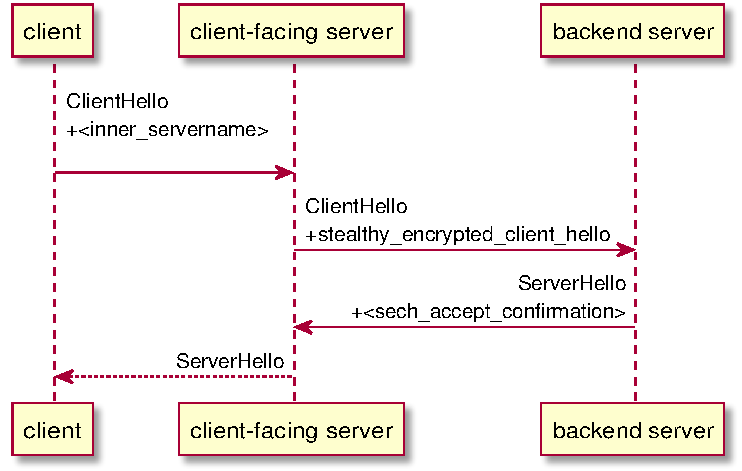
\includegraphics[width=\linewidth]{figure/sech-split-mode-accept.pdf}
\captionsetup{width=.8\linewidth} 
\caption[]{Sequence diagram for a successful SECH split-mode handshake.}
\label{fig:sech-split-mode-accept}
\end{figure}

\section{SECH 1: Secretless Stealthy Encoding}
\subsection{Motivations and Deployment Scenarios}

[ ] more properly should be called just `stealthy SNI' or `stealthy CH', because this version does not use encryption

[ ] very low coordination/infrastructure requirements to get this working

[ ] SECH.1 does **not** offer confidentiality of the SNI or ALPN, aim here is purely censorship circumvention, not privacy

[ ] as a censorship circumvention method this can be easily detected and prevented

[ ] possibly useful ephemerally and at a small scale

[ ] circumvention in depth: use lots of different circumvention methods (including this insecure one) in order to increase the cost of censorship
\subsection{Design}
\subsection{Implementation Notes}


\section{SECH 2: Static Secret Shared OOB}
\subsection{Motivations and Deployment Scenarios}

The amount of `cover' available in the TLS 1.3 \var{ClientHello} message in which we can hide information without differentiating the message from an a normal TLS 1.3 message is limited. By using only a symmetric encryption algorithm as the basis for sending the stealthy information there is a smaller overhead than there would be with PKC or HPKE.

With the \var{random} and \var{legacy\_session\_id} fields we get a contiguous sequence of 64 octets. Other fields/extensions with values that {\em may} look random (and thus might provide cover) are the cipher suite GREASE values, the PSK identity, the \var{key\_share} itself. However, the cover provided by these fields/extensions would be less certain because they differ across situations/implementations of TLS. Using these effectively as cover for stealthy bits would involve mimicking the behaviour of a specific implementation in order not to stick out.

[ ] if the client and server can share the OOB secret securely then we can implement a highly stealthy and cryptographically secure inner SNI

[ ] since the server does not have to publish a public key (as in ECH), it is possible to hide the fact that the server is support SECH from all except the client who knows the OOB secret

[ ] the secret could be shared amongst multiple clients, allowing for some scale of deployment, but this protocol is certainly not appropriate for internet scale deployments (millions of clients). The more widely the secret is shared the more likely it is to be leaked.

[ ] This design is NOT forward secret. If the shared secret is compromised then 

\subsection{Design}

We assume the client and client-facing server have some way to securely share a secret out-of-band; call this secret $s$ or \var{sech2\_long\_term\_key}. The shared secret should be a random string of at least 32 octets, or a longer string with at least that much entropy.


The client wishes to communicate \var{sech\_inner\_servername} secretly and stealthily to the client-facing server. Due to the limited amount of `cover' in the \var{ClientHello} the maximum length of \var{sech\_inner\_servername} is \sechtwoservernamelen. The \var{sech\_inner\_servername} is padded with a suffix of zeros to yield \var{padded\_servername} which is \sechtwoservernamelen octets long.  The client also generates a session-specific \sechtwoivlen{} octet \nonce. The plain text for encryption $pt$ is the \sechtwoservernamelen{} octet \var{padded\_servername}.
The session SECH 2 encryption key $sk_c$=\var{sech\_session\_secret} is computed as defined in \ref{lst:sech2-derive-secret}.
The client should ensure that it has never used the $(\nonce,sk_c)$ pair before, but ensuring that $(\nonce,sk_c)$ are never reused globally may not be feasible. Ideally the $(\nonce,sk_c)$ should never be used twice by any clients, but if there a multiple clients that do not coordinate this will be impossible to guarantee.


We note that the \var{random} and \var{legacy\_session\_id} are contiguous giving us a contiguous string of 64 octets in which we hide the SECH 2 offer, and we call this contiguous string $c$ for `cover'. The AEAD encrypted text has length \sechtwocipherlen{} and is placed in bytes \sechtwocipheroffset{}  to \sechtwocipherend{} of $c$, as depicted in Figure~\ref{fig:sech2-cover}, yielding \var{\ClientHelloOuter}.

We define \var{ClientHelloOuterContext} as a clone of \var{ClientHelloOuter}, except with bytes 12 to 64 of the cover $c$ set to 0s. The session key $sk_c$ can only be computed after \var{Client\-HelloOuterContext} is known.
The secure derivation of $sk_c$ depends on the entropy of the \var{key\_share} extension included in \var{ClientHelloOuterContext}.
[ ] TODO: what if key\_share is not included, e.g. for PSK-only handshake? Reject SECH?

The additional authenticated data $aad$ is empty.

%the transcript of \var{ClientHelloInner} message, which is \var{ClientHelloOuter} but with: 1. the encrypted AEAD output replaced with the plain text \var{sech\_inner\_servername} and \var{sech\_inner\_random}, as well as 2. the \var{extension\_data} field of the \var{server\_name} extension set to all 0s with the same length as the cover value for \var{server\_name} (The backend server does not learn the cover SNI used). The AEAD MAC $t$ is left in \var{ClientHelloInner}.

\begin{listing}[htb]
\centering
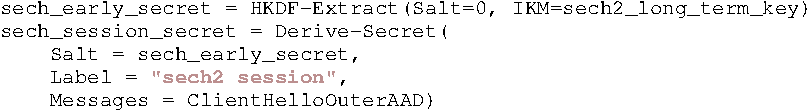
\includegraphics[width=\linewidth]{figure/sech2-derive-secret.pdf}
\captionsetup{width=.8\linewidth} 
\caption[SECH 2 Derive Secret]{Derive $sk_c$, the secret key that will be used by the client to encrypt $pt$ which has the inner \var{CH} data.}
\label{lst:sech2-derive-secret}
\end{listing}

The client encrypts $pt$ (authenticating $aad$) with $(\nonce,sk_c)$ using AES-128-GCM, producing a \sechtwotaglen{} octet authentication tag $t$ and the \sechtwocipherlen{} octet encrypted text $ct$. The \var{\ClientHelloOuter} has $c:=\nonce||ct||t$. The placement of the required values in cover $c$ of the \var{\ClientHelloOuter} is depicted in Figure~\ref{fig:sech2-cover}.

\begin{figure}[htb]
\centering
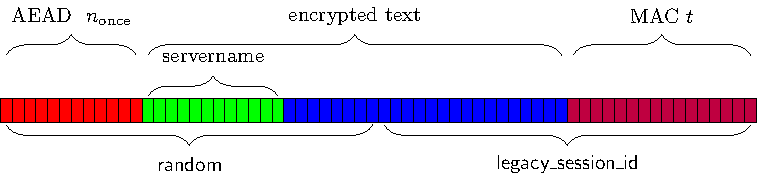
\includegraphics[width=\linewidth]{figure/sech2-cover.pdf}
\captionsetup{width=.8\linewidth} 
\caption[SECH 2 Cover]{Locations of AEAD inputs and outputs in the 64 contiguous octets of \var{ClientHello} \var{random} and \var{legacy\_session\_id}. The cipher text $ct$ and MAC tag $t$ outputs are a function of $iv$, $s$, $pt$, and $aad$: $(ct,t)=\text{AEAD}(iv,s,pt,aad)$.}
\label{fig:sech2-cover}
\end{figure}

A cooperating server in possession of $s$ that receives a \var{ClientHello} first constructs \var{ClientHelloOuterContext}, then $sk_c$, and should attempt to decrypt and authenticate $ct$. If decryption/authentication are unsuccessful the server continues with the TLS 1.3 handshake as normal. If successful, the client-facing server forwards \var{ClientHelloInner} to the backend server identified by the inner server name. If the inner server name does not identify a backend server then the client-facing server continues the TLS 1.3 handshake as if SECH 2 is disabled.

The \var{ClientHelloInner} message  is \var{ClientHelloOuter} but with: 1. the encrypted AEAD output $ct$ replaced with the plain text $pt$, as well as 2. the \var{extension\_data} field of the \var{server\_name} extension set to all 0s with the same length as the cover value for \var{server\_name} (The backend server does not learn the cover SNI used). The AEAD MAC $t$ is left in \var{ClientHelloInner}.

The backend server can distinguish a \var{ClientHelloInner} from a regular regular \var{ClientHello} by the \var{server\_name} extension. If the \var{extension\_data} field of the \var{server\_name} has all 0s it is a \var{ClientHelloInner}. Otherwise it should be treated as a regular TLS 1.3 hello.

The server parses the plaintext $pt$ to retrieve the inner server name in order to select an identity. At this point the backend server might respond with \var{HRR} or \var{ServerHello}. Whereas in ECH the acceptance signal is always sent in the server's first message (whether it is a \var{HRR} or \var{SH}), for SECH 2 the acceptance signal is always in the \var{SH}. The client-facing server forwards these (and subsequent) messages to the client unaltered. In the case of \var{HRR} the backend server creates a normal \var{HRR} response and the client constructs \var{ClientHello2} as specified in RFC 8446 (\cite{rfc8446}). If the backend server accepts the parameters of \var{ClientHello} (or \var{ClientHello2} in the case of \var{HRR}) and accepts the inner servername identified in $pt$, then it responds with a special \var{ServerHello} containing an SECH acceptance signal. Also, if using certificate-based authentication, then the later \var{Certificate} message should contain a certificate identified in $pt$.

The SECH 2 acceptance signal is 8 octets long and placed in the last 8 bytes of the \var{ServerHello.random}. It is a function of the transcript of the handshake so far, \var{sech\-\_\-transcript\_hash}, and $s=$\var{sech2\_long\_term\_key}. We define \var{sech\_accept\_confirmation} in Listing~\ref{lst:sech2-accept-function} and \var{sech\_transcript\_hash} in Listing~\ref{lst:sech2-transcript-hash}.

\begin{listing}[htb]
\centering
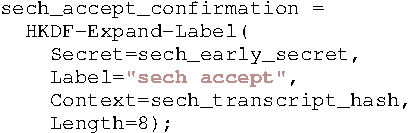
\includegraphics[width=.7\linewidth]{figure/sech2-accept-function.pdf}
\captionsetup{width=.8\linewidth} 
\caption[SECH 2 Accept Confirmation]{The function used to calculate the SECH 2 acceptance signal using the \var{HKDF-Expand-Label} function defined in Section 7.1 of RFC 8446 (\cite{rfc8446}). The \var{sech\_early\_secret} is derived from $s$ as defined in Listing~\ref{lst:sech2-derive-secret}, and \var{sech\_transcript\_hash} is described in Listing~\ref{lst:sech2-transcript-hash}.}
\label{lst:sech2-accept-function}
\end{listing}

\begin{listing}[htb]
\centering
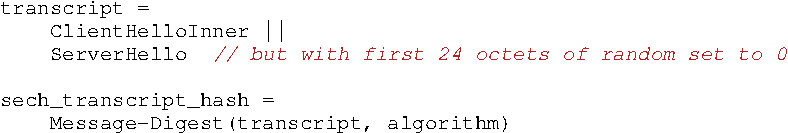
\includegraphics[width=\linewidth]{figure/sech2-transcript-hash.pdf}
\captionsetup{width=.8\linewidth} 
\caption[SECH 2 Transcript Hash]{Specification of the \var{sech\_transcript\_hash} used to calculate \var{sech\_accept\_confirmation}. The \var{algorithm} is the hash algorithm of the negotiated cipher suite for the handshake.}
\label{lst:sech2-transcript-hash}
\end{listing}

% The client uses that secret to encrypt the true target servername as well as a 32 byte secret inner nonce which are hidden in the ClientHello \var{random} and the \var{pre\_shared\_key} extension. The inclusion of the secret inner nonce is necessary to mitigate cut-and-paste attacks.

% More precisely, the client generates a 12 byte initialisation vector for AES-128-GCM. The plaintext is an ASCII encoding of the servername padded with 0x00 up to 12 bytes, appended to the 32 byte inner nonce.
% AEAD is used but the AAD is 0-length. % TODO: might be better to use the transcript hash of ClientHello (with random zeroed) as AAD, (however, if random is zeroed then transcript hash might not change)
% The AEAD tag is truncated to 8 bytes, such that we have a combined 64 bytes to send, which are put into the \var{ClientHello.random} and \var{ClientHello.legacy\_session\_id}. The first 12 bytes contain the IV, the next 12 contain the first 12 bytes of the cipher text, and the last 8 bytes of the \var{random} contain the truncated MAC, and the \var{ClientHello.legacy\_session\_id} is the last 

If the backend server accepts SECH 2 then it makes the SECH inner servername available to the application program via a callback or some other means, which allows the application program to decide whether or not to switch contexts (server certificate etc.).

\subsubsection{SECH 2 with PSK}
If a server accepts SECH 2 it may issue a ticket referencing a PSK that can be used to resume with backend server without stealthy encryption.

The PSK is derived as defined in Listing~\ref{lst:sech2-psk}, which differs from the definition of the PSK defined RFC 8446 in that the label is \var{``sech res''} rather than \var{``resumption''}. This ensures that the standard TLS 1.3 PSK is only used for a connection to the outer servername, whereas the \var{sech2\_psk} is only used for the inner servername.
\begin{listing}
\begin{verbatim}
sech2_psk = HKDF-Expand-Label(
    resumption_master_secret,
    "sech res",
    ticket_nonce,
    Hash.length)
\end{verbatim}
\caption{\label{lst:sech2-psk}Definition of the PSK used when resuming an SECH 2 session.}
\end{listing}

Note that this definition of \var{sech2\_psk} is a function of the \var{resumption\_master\_secret}, which is not available to a client-facing server in split-mode.
Therefore, this type of resumption is not possible in split-mode. % TODO: design PSK resumption for split mode
% TODO: what if sech2_psk and psk are the same, e.g. because they collide when using different ticket_nonces? maybe the label should still be "sech res" but each ticket_nonce should be marked as either sech or non-sech?

To use a resumption PSK (sent via \var{NewSessionTicket}) in TLS 1.3 the PSK has to be validated with a \var{BinderEntry} which binds the PSK cryptographically to the transcript of the first handshake as well as most of the \var{CH} for the second handshake. Pseudocode for this process is presented in Listing~\ref{lst:binder-pseudocode}, but this process is not used in SECH 2, as explained below.

\begin{listing}
    \begin{verbatim}
early_secret = HKDF-Extract(0, PSK)
binder_key = Derive-Secret(early_secret, "res binder", "")
binder_finished_key = HKDF-Expand-Label(
    binder_key,
    "finished",
    "",
    Hash.length)
binder =
    HMAC(binder_finished_key,
        Transcript-Hash(
            HandshakeContext1..ClientHello))
    \end{verbatim}
    \captionsetup{width=.8\linewidth} 
    \caption{\label{lst:binder-pseudocode}Pseudocode of the process used to compute a \var{binder} when using a resumption PSK. The \var{HandshakeContext1} is the transcript of the handshake in which the PSK was derived, and \var{ClientHello} is for a new connection and is truncated so as not to include the \var{binders} list itself. This formulation is tweaked slightly in the case of SECH 2.}
\end{listing}

\subsection{Distributing SECH 2 access without sharing \var{sech2\-\_long\-\_term\_secret}}
[ ] TODO research has anyone done ticket sharing amongst clients before? E.g. client with multiple processes

[ ] TODO bleichenbacher attack

Sharing the SECH 2 long term secret widely amongst clients would violate the `Avoid Widely Shared Secrets' requirement advocated by \citep{rfc8744-issues}. How do we facilitate connections from large numbers of clients while restricting each long term secret to being shared to only 2 parties? One option is to have a distinct long term secret for each client-server pair. The SECH 2 design specified here can facilitate this through trial decryption, i.e. every \var{ClientHello} processed by the server is checked against each registered secret until one is found to successfully decrypt the inner server name. This approach scales horribly, with the cost of every connection being proportional to the number of registered clients, whether or not those clients are active. But note that this trial decryption process is highly parallelizable.

Another approach is to modify the TLS 1.3 session resumption mechanism in order to allow a client to distribute PSKs to other clients. Those other clients could then resume the first client's session in order to access the backend server.

When a servers generates a \ac{PSK} and shares it in a \ac{NST} message, then (in TLS 1.3) \ac{PSK} is of type ``resumption'', rather than ``external''. Using ``resumption'' tickets/\acp{PSK} has a few extra steps compared to ``external'' \acp{PSK}. The calculation of the \var{binder} when using ``resumption'' incorporates the transcript of messages from the first session as well as initial messages from the new session, whereas without an external \ac{PSK} there is no `first' session so the transcript is just of the first session.

We consider now the scenario where a client (C1) completes an SECH 2 handshake in order to establish a PSK, but wishes to pass the PSK to a different client (C2) so that C2 can connect to the backend server stealthily without knowing the \var{sech2\_long\_term\_key}. One approach would be to treat the \ac{PSK} as ``resumption'' type. This would require the \var{binder} value in Listing~\ref{lst:binder-pseudocode} which is a function of the PSK and the transcript up to and including the new \var{ClientHello}. For resumption \acp{PSK} \var{Handshake Context 1} is the transcript of the first session's handshake, whereas for external \acp{PSK} \var{Handshake Context 1} is the empty string. Typically the \var{HandshakeContext1} is private because it contains decrypted confidential handshake messages, and therefore should not be shared with the other untrusted client C2. At the same time, in order to compute a valid \var{ClientHello} the private component of the \var{key\_share} is needed, and this value should not be accessible to C1 when C2 is resuming the session. In other words C1 should have exclusive access to the first part of the transcript, and C2 must generate the second part of the transcript. Therefore, in order to calculate the \var{binder} while maintaining these rules C2 would have to send the new \var{ClientHello} to C1. This is highly inconvenient operationally; it means that C1 would have to remain live and accessible in order for C2 to use the \ac{PSK}. For these reasons we deem that using \acp{PSK} of type ``resumption'' to bootstrap a second client is not viable.

\begin{listing}
    \begin{verbatim}
binder =
    HMAC(binder_key,
        Transcript-Hash(Handshake Context1,
        ClientHello) )
    \end{verbatim}
    \captionsetup{width=.8\linewidth} 
    \caption{\label{lst:binder-sech2-pseudocode}Normal calculation of \var{binder} in TLS 1.3.}
\end{listing}

While binding the bootstrap \ac{PSK} to the session in which it was generated is desirable, and it would be more congruent with the existing TLS 1.3 spec (\acp{PSK} delivered by \ac{NST} are bound in this way), we instead opt to treat bootstrap \acp{PSK} more like `external' keys. The calculation of the \var{binder} is simplified as in Listing~\ref{lst:binder-sech2-pseudocode-ext}. By acquiring from C1 just the \ac{PSK} value itself and the associated hash algorithm C2 has enough information to use the \ac{PSK}.

\begin{listing}
    \begin{verbatim}
binder =
    HMAC(binder_key,
        Transcript-Hash(ClientHello))
    \end{verbatim}
    \captionsetup{width=.8\linewidth} 
    \caption{\label{lst:binder-sech2-pseudocode-ext}Calculation of \var{binder} for SECH 2 bootstrap \acp{PSK}.}
\end{listing}

%[ ] The server uses the 32 byte shared secret key as well as the decrypted inner servername to create an 8 byte acceptance signal which is hidden in the ServerHello.random. The 8 byte acceptance signal is computed as \var{sech\_accept\_confirmation = AEAD-encrypt(IV, plaintext="", aad=sech\_inner\_servername, accept\_key).tag}, where IV is the first 12 bytes of the ServerHello.random (uniformly randomly generated), the plaintext is zero-length, the AAD is precisely the inner servername (which does not need to be transmitted because it is known by the client), and \var{accept\_key} is a session-specific key derived using HKDF from the session's master secret and the transcript of ClientHello..ServerHello, but with the last 16 bytes of ServerHello.random set to 0x00. The last 8 bytes of \var{ServerHello.random} are possibly used for an ECH acceptance signal, and the ECH acceptance signal is computed based on the transcript of ClientHello..ServerHello, except with the last 8 bytes of of ServerHello.random set to 0x00. Therefore, if the server is sending an SECH acceptance signal *and* an ECH acceptance signal, the SECH acceptance signal is computed first because the ECH acceptance signal is defined to incorporate the SECH acceptance signal bytes in its transcript hash. To construct the 8 sech\_accept\_confirmation bytes we make use of the HKDF-Expand-Label function defined in RFC 8446 Section 7.1.
    % ```c
    % md = TranscriptHash(ClientHello..ServerHello) // with last 16 bytes of ServerHello.random set to 0x00
    % padded\_sech\_IV = pad(sech\_IV, HashLen)
    % sech\_accept\_confirmation = HKDF-Expand-Label(
    %   HKDF-Extract(padded\_sech\_IV, sech\_symmetric\_key),
    %   "sech ac" || 0x00 || sech\_decrypted\_inner\_servername,
    %   md,
    %   8
    % )
    % ```

\subsection{Design Differences Between SECH 2 and ECH}
[ ] The acceptance signal is always sent in the \var{ServerHello}

[ ] This definition of \var{sech\_accept\_confirmation} is essentially a modification of the ECH \var{accept\_confirmation} defined in Section 7.2 of [TODO cite ECH draft], which we repeat here:
% ```
%   accept\_confirmation = HKDF-Expand-Label(
%     HKDF-Extract(0, ClientHelloInner.random),
%     "ech accept confirmation",
%     transcript\_ech\_conf,
%     8
%   )
% ```

The ECH \var{accept\_confirmation} uses \var{HKDF-Extract(0, ClientHelloInner.random)} as the `Secret' passed to \var{HKDF-Expand-Label}, and \var{HKDF-Extract(0,ClientHelloInner.random)} is confidential (only known to the client and server) because the \var{ClientHelloInner.random} was in the {\em encrypted} \var{ClientHelloInner}. Also, it is essential that \var{accept\_confirmation} can be generated by the backend server in ECH split mode, which is why the salt passed to \var{HKDF-Extract} is the 0 string. While it would be more secure to use a session-specific random value as the salt for \var{HKDF-Extract}, we cannot use the \var{ClientHelloOuter.random} because this value is not available to the backend server (the backend server only processes the ClientHelloInner). The HKDF specification assumes that the salt and IKM passed to HKDF-Extract are indepedent of each other (Section 3.4 RFC 5869), and in particular that the salt values are not `chosen or manipulated by an attacker'.
Since \var{ClientHelloOuter.random} is never processed by the backend server it will not be incorporated into the \var{Finished} message, which means it is not protected from tampering in split-mode. This means an attacker could manipulate \var{ClientHelloOuter.random} and so it should not be used as the salt for \var{HKDF-Extract}.

[ ] In order to facilitate a split mode of operation in a similar fashion to ECH it must be possible for the SECH backend server to produce  the \var{sech\_accept\_confirmation} signal. For the signal described above this entails that the backend server must possess the \var{sech\_symmetric\_key}, meaning \var{sech\_symmetric\_key} would be shared amongst three parties; client, client-facing server, backend server. This violates one of the design requirements listed in Section 3.2 by \cite{rfc8744-issues}; Avoid Widely Shared Secrets.
% \subsection{Security Considerations}

[ ] High probability for situations where an attacker can guess the plaintext, or where there are only a small number of possible plaintexts (SNIs). How does this affect capacity to brute force the secret key? -> Does this mean the SNIs must also remain secret?

\subsection{Implementation Notes}

[ ] Error handling
\subsection{Testing}

\section{SECH 3}
\subsection{Motivations and Deployment Scenarios}
\subsection{Design}
\subsection{Implementation Notes}
\section{SECH 4}
\subsection{Motivations and Deployment Scenarios}
\subsection{Design}
\subsection{Implementation Notes}

\section{SECH 5}
\subsection{Motivations and Deployment Scenarios}

[ ] arbitrary access for new clients without coordination from server

\subsection{Design}

[ ] server produces an \var{SECHConfig} and corresponding private key for the KEM

[ ] client has to attain \var{SECHConfig} in order to offer SECH 5 in a \var{ClientHello}, can attain over DoH or some other means

[ ] client encapsulates an ephemeral key $k$ using the KEM and public key specified in \var{SECHConfig} producing \var{enc}

[ ] client pads the servername to \var{SECHConfig.servername\_length} producing \var{\paddedServername}

[ ] client encrypts the \var{padded\_servername} with the AEAD specified in SECHConfig, and with key $k$ and a \nonce which is the first 12 octets of the hash of \var{SECH5ClientHelloAAD}, and with \var{SECH5ClientHelloAAD} as AAD, producing \var{sech5\_cipher} which is the concatenation of the encrypted text and the tag $t$

[ ] \var{SECH5ClientHelloAAD} is the \var{ClientHello} but with the portion in which the AEAD cipher (encrypted text and tag) will be placed set to zero, the size and location of this region depends on \var{SECHConfig}

[ ] \var{SECH5ClientHelloAAD} is the \var{ClientHelloOuter} but with the \var{random} and \var{legacy\_session\_id} set to all 0s

[ ] client encodes \var{enc} and \var{sech5\_cipher} in the \var{ClientHello} \var{random} and \var{legacy\_session\_id} fields producing \var{ClientHelloOuter} as depicted in Figure~\ref{fig:sech5-cover}

[ ] the client-facing server attempts to decapsulate \var{enc} with the private key associated with \var{SECHConfig} retrieving $k$, on failure continues with normal TLS 1.3

[ ] the client-facing server computes \var{SECH5ClientHelloAAD} and the \nonce, and then attempts to decrypt $ct$ and authenticate with $t$, on failure continues with normal TLS 1.3

[ ] on success the client-facing server constructs \var{SECH5ClientHelloInner} by replacing $ct$ with $pt$ and setting the \var{extension\_data} of the \var{server\_name} extension to all 0s

[ ] client-facing server forwars \var{SECH5ClientHelloInner} to the backend server

[ ] the backend server proceeds with SECH 5 iff the \var{server\_name} extension has all 0s, otherwise continues with normal TLS 1.3

[ ] the backend server might respond with \var{HRR} or \var{ServerHello}, the \var{HRR} is constructed as normal, but the \var{ServerHello} contains a special \var{sech5\_accept\_confirmation} value in the last 8 octets of the \var{random}


\begin{figure}[htb]
\centering
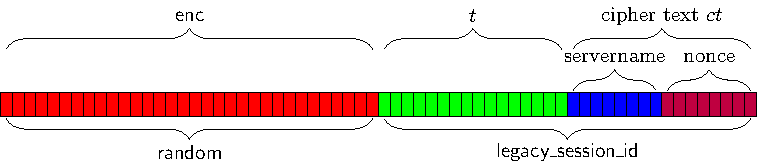
\includegraphics[width=\linewidth]{figure/sech5-cover.pdf}
\captionsetup{width=.8\linewidth} 
\caption[SECH 5 Cover]{}
\label{fig:sech5-cover}
\end{figure}

\subsection{Implementation Notes}

\section{SECH 6: TLS over TLS}
\subsection{Motivations and Deployment Scenarios}
\subsection{Design}
\subsection{Implementation Notes}


% At the beginning of each chapter, a description should introduce the reader to the content of the chapter. The description should explain to the reader the layout of the chapter, the contribution that the chapter makes to the overall dissertation and the contribution of the individual sections towards the overall chapter.


% \section{Problem Formulation}
% \label{sec:ProblemFormulation}

% This section should provide the reader with an overall description of the problem that will be addressed in the dissertation. In contrast to a generic discussion of the dissertation topic in the Introduction chapter, this section should provide a detailed discussion of the problem that has been identified based on the existing work that has been discussed in the preceeding chapter. 

% In some dissertations, it may make sense to convert this section into a short chapter of its own which follows the discussion of the existing work and preceeds the discussion of the work of the dissertation.

% \subsection{Identified Challenges}
% This section should present a short description of the gaps in the existing work and the relationship of these gaps to the work described in this dissertation.

% \subsection{Proposed Work}
% This section should provide a thorough description of the problem and an overview of the work proposed to address the problem.


% \section{Overview of the Design}
% \label{sec:OverviewOfDesign}
% A description of the approach that addresses the problem identified above.


% \section{Summary}
% \label{sec:SummaryDesign}

% Every chapter aside from the first and last chapter should conclude with a summary. 

\chapter{Implementation, Testing, and Deployment}

\section{Implementing an SECH API in OpenSSL}
\subsection{Introduction}
\subsection{Testing}
\subsection{Conclusions}
\section{Test Deployment}
\subsection{Introduction}
\subsection{Methods}
\subsection{Results}
\subsection{Discussion}

% \lstset{language=Python, captionpos=b, frame=single}
% \captionsetup{width=.8\linewidth} 


% Guess what? At the beginning of each chapter, a description should introduce the reader to the content of the chapter. The description should explain to the reader the layout of the chapter, the contribution that the chapter makes to the overall dissertation and the contribution of the individual sections towards the overall chapter.


% \section{Overview of the Solution}

% %% Short caption for the table of listings - long caption for the explanation for the reader
% \includecode{Sample Code}{Lengthy caption explaining the code to the reader}{lst:snippet}{snippet.py}

% The code in listing~\ref{lst:snippet} is a demonstration how to include a file with code into the template.



% \section{Component One}

% %% Defaults for listings

% The code in listing~\ref{lst:snippet2} is a demonstration how to include code in the template.

% %% Short caption for the table of listings - long caption for the explanation for the reader
% \begin{lstlisting}[caption={[Sample Code 2]Second Lengthy caption}, label={lst:snippet2}]
% x = 1
% if x == 1:
%     # indented four spaces
%     print("x is 1.")
% \end{lstlisting}


% \section{Summary}

% Every chapter aside from the first and last chapter should conclude with a summary. 


\chapter{Evaluation}
\label{chap:Evaluation}

\section{General Security and Privacy Considerations for SECH}

\subsection{Protocol Confidentiality}
As mentioned in Section~\ref{bleichenbacher-attack} any good \ac{SECH} protocol should protect the confidentiality of the fact that \ac{SECH} is being attempted and the fact that \ac{SECH} is supported. There are aspects of the protocol design that will protect this information, for instance how the connection continues with regular \ac{TLS} 1.3 whenever \ac{SECH} is aborted.
However, ensuring the confidentiality of this information depends also on
a careful and secure information. For instance, it may be possible for an attacker to somehow with high likelihood guess the library/implementation used for a particular channel. With this information the attacker could then analyse the timing of messages, or the particular alert messages under various circumstances to gain information about whether \ac{SECH} is in use.
The recurring discovery of \ref{bleichenbacher-attack}-style attacks are an attestation to the difficulty of implementing protocols that do not reveal such secret information.

To make matters worse, unlike \ac{RSA} private messages/keys which consist of many bits, the fact of a protocol being used/supported can be represented by a single bit, so protocol confidentiality is broken if an attacker can attain this single bit, meaning a successful attack will likely require much fewer oracle accesses than is the case for \ref{bleichenbacher-attack}. It should not be taken for granted that any given implementation of \ac{SECH} sufficiently protects protocol confidentiality.

% The Evaluation chapter should present a comparison of the work that forms the basis of the dissertation and existing work. At a higher level, it should demonstrate an awareness of the relationship of the dissertation work to the research area that it is based in.

% \section{Experiments}

% In the case where experiments have been carried out, the experimental setup and the values that were defined for the variables need to be presented in a table e.g. table~\ref{tab:experimentsetup}.

% \begin{table}[!h]
% \begin{center}
% 	\begin{tabular}{|l|c|c|} 
% 	\hline
%  	\bf Column 1  & \bf Column 2  & \bf Column 3 \\
%   	\hline
% 	Row 1 & Item 1 & Item 2 \\
% 	Row 2 & Item 1 & Item 2 \\
% 	Row 3 & Item 1 & Item 2 \\
% 	Row 4 & Item 1 & Item 2 \\
% 	\hline
% 	\end{tabular}
% \end{center}
% \caption[Variables of the experiment]{Caption that explains the table to the reader}	
% \label{tab:experimentsetup}
% \end{table}


% \section{Results}

% Figures that present results such as figure~\ref{fig:measurements} need to display descriptions of the axes, the units and scales of the measurements, statistical values, etc. Where measurements were taken from experiments, error bars or confidence intervals need to be provided to give the reader an indication of the spread of the measurements.

% \includescalefigure{fig:measurements}{Measurement of System Wakeups}{Long caption that describes the figure to the reader}{1}{measurements.png}


% \section{Summary}

% Every chapter aside from the first and last chapter should conclude with a summary that presents the outcome of the chapter in a short, accessible form. 
\chapter{Conclusions \& Future Work}
\label{chap:Conclusions}


\section{Future Work}

% This chapter should summarize the work presented in the dissertation and discuss the conclusions that can be drawn from the work and the results presented in chapter~\ref{chap:Evaluation}.


% \section{Future Work}

% The section may present a list of items that were beyond the scope of the dissertation.

% \begin{thebibliography}{refs}                   %% Start your bibliography here; you can
\addcontentsline {toc}{chapter}{Bibliography}     %% Force Bibliography to appear in contents
\bibliographystyle{apalike}
\bibliography{refs}                               %% also use the \bibliography command
%\end{thebibliography}                            %% to generate your bibliography.


%\addcontentsline {toc}{chapter}{Appendices}       %% Force Appendices to appear in contents
%\begin{appendix}
%\include{appendix1}
% \include{appendix2}
%\end{appendix}




\end{document}                                    %% END THE DOCUMENT
